\documentclass[conference,a4paper]{IEEEtran}
\usepackage[T1]{fontenc}
\usepackage[utf8]{inputenc}
\usepackage{cite}
\usepackage[hidelinks]{hyperref}
\usepackage{float}
\usepackage{array}
\usepackage{booktabs}
\usepackage{graphicx}
\usepackage{listings}
\usepackage{xcolor}
\usepackage{tikz}
\usetikzlibrary{arrows.meta, positioning}

\graphicspath{{images/}}

% ── Code listing style ──────────────────────────────────────────────────────
\definecolor{codegray}{rgb}{0.95,0.95,0.95}
\definecolor{codegreen}{rgb}{0.13,0.47,0.24}
\definecolor{codeblue}{rgb}{0.13,0.29,0.53}
\definecolor{codegrey2}{rgb}{0.4,0.4,0.4}

\lstset{
  backgroundcolor=\color{codegray},
  basicstyle=\ttfamily\scriptsize,
  keywordstyle=\color{codeblue}\bfseries,
  stringstyle=\color{codegreen},
  commentstyle=\color{codegrey2}\itshape,
  breaklines=true,
  frame=single,
  framesep=4pt,
  xleftmargin=6pt,
  xrightmargin=6pt,
  aboveskip=6pt,
  belowskip=6pt,
  showstringspaces=false,
  tabsize=4,
  captionpos=b,
}

\lstdefinelanguage{CQL}{
  morekeywords={CREATE,TABLE,IF,NOT,EXISTS,PRIMARY,KEY,WITH,CLUSTERING,
                ORDER,BY,DESC,ASC,TEXT,TIMESTAMP,DOUBLE,INT,LIST,KEYSPACE},
  keywordstyle=\color{codeblue}\bfseries,
  morestring=[b]',
  stringstyle=\color{codegreen},
}

% ── Title ───────────────────────────────────────────────────────────────────
\title{Real-Time IoT Weather Monitoring System\\
{\large Final Report --- Internet of Things}}

\author{%
\IEEEauthorblockN{Eljon Shala}
\IEEEauthorblockA{%
Department of Computer and Software Engineering\\
Faculty of Electrical and Computer Engineering\\
University of Prishtina\\
Prishtina, Kosovo\\
eljon.shala@student.uni-pr.edu}
\and
\IEEEauthorblockN{Brahim Sylejmani}
\IEEEauthorblockA{%
Department of Computer and Software Engineering\\
Faculty of Electrical and Computer Engineering\\
University of Prishtina\\
Prishtina, Kosovo\\
brahim.sylejmani@student.uni-pr.edu}
}

% ========================================================================
\begin{document}
\maketitle

\begin{abstract}
This report documents the design and implementation of a complete, end-to-end
Internet of Things (IoT) system for real-time weather monitoring across three
stations in Kosovo. The system collects, transports, processes, stores, and
visualizes weather sensor data using a modern big-data streaming pipeline.
Since physical sensors are unavailable, a physics-based simulator was developed
to generate realistic meteorological readings including seasonal cycles, diurnal
temperature swings, correlated storm events, and injected sensor anomalies.

Data is streamed through Apache Kafka, processed in real time by Apache Spark
Structured Streaming, and stored in Apache Cassandra. A Flask web dashboard
provides live visualization with five parameter charts, a real-time alert
system, an AI insights panel, and a downloadable PDF report. Three advanced
components --- a local AI module with three machine learning models, a real-time
alerting system embedded in Spark, and a performance benchmarking suite --- were
implemented for exam exemption. The entire system is containerized with Docker
Compose and starts with a single command.
\end{abstract}

\begin{IEEEkeywords}
IoT, Apache Kafka, Apache Spark Streaming, Apache Cassandra, real-time monitoring,
weather monitoring, machine learning, alerting, Docker
\end{IEEEkeywords}

% ========================================================================
\section{Introduction}

This is the second part of the IoT project. Part~1 covered the theoretical
foundations of IoT systems --- sensor types, communication protocols (MQTT,
HTTP, CoAP), and architectural models. This report focuses entirely on the
practical implementation using the technology stack prescribed by the professor.

The core objectives are:
\begin{itemize}
  \item Build a physics-based weather simulator modelling realistic meteorological dynamics for three Kosovo stations.
  \item Use Apache Kafka as a high-throughput, fault-tolerant message broker, with a producer and two independent consumers.
  \item Use Apache Spark Structured Streaming to perform data validation, raw ingestion, sliding-window aggregations, and threshold-based alerting concurrently.
  \item Store all data in Apache Cassandra across five optimized tables.
  \item Provide a live web dashboard with charts, windowed-aggregate trends, AI insights, alerts, and PDF export.
  \item Implement three advanced components for exam exemption: AI, alerting, and performance analysis.
  \item Containerize every service so the full stack starts with \texttt{docker-compose up}.
\end{itemize}

% ========================================================================
\section{Project Infrastructure and Architecture}

\subsection{System Components}

The system is a microservices pipeline. Each component is an independent,
containerized Docker service:

\begin{enumerate}
  \item \textbf{Data Producer} (\texttt{data\_producer/}): Runs the \texttt{WeatherSimulator} class and publishes JSON readings to Kafka every 2~seconds.
  \item \textbf{Apache Kafka + Zookeeper}: Message broker decoupling producers from consumers. Hosts two topics: \texttt{weather\_data} and \texttt{weather\_alerts}.
  \item \textbf{Apache Spark Streaming} (\texttt{spark\_processor/}): The primary consumer of \texttt{weather\_data}; runs two concurrent streaming queries (with a validation stage) and writes to Cassandra.
  \item \textbf{Alerts Consumer} (\texttt{alerts\_consumer/}): A second, independent consumer subscribed to \texttt{weather\_alerts}; routes critical alerts to a notification dispatch and logs warnings.
  \item \textbf{Apache Cassandra}: Distributed NoSQL database storing five tables.
  \item \textbf{setup-cassandra}: One-shot container that creates the schema before data flows in.
  \item \textbf{ai-trainer}: One-shot container that generates one year of synthetic history and trains three ML models.
  \item \textbf{Dashboard} (\texttt{dashboard/}): Flask web application serving live charts, windowed-aggregate trends, AI insights, alerts, and PDF export.
\end{enumerate}

\subsection{Data Flow}

\begin{figure}[H]
\centering
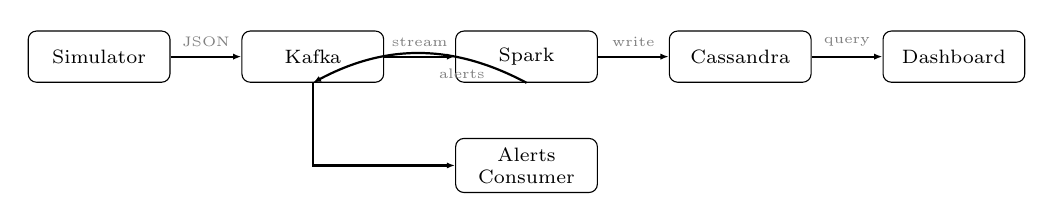
\begin{tikzpicture}[
  node distance=0.55cm and 0.9cm,
  every node/.style={font=\scriptsize},
  box/.style={draw, rectangle, rounded corners=3pt, minimum width=1.8cm,
              minimum height=0.65cm, align=center},
  arrow/.style={-{Latex[length=3pt]}, thick},
  lbl/.style={font=\tiny, color=gray},
]
\node[box] (sim)   {Simulator};
\node[box, right=of sim]   (kafka) {Kafka};
\node[box, right=of kafka] (spark) {Spark};
\node[box, right=of spark] (cass)  {Cassandra};
\node[box, right=of cass]  (dash)  {Dashboard};
\node[box, below=0.7cm of spark] (cons) {Alerts\\Consumer};

\draw[arrow] (sim)   -- node[lbl,above]{JSON} (kafka);
\draw[arrow] (kafka) -- node[lbl,above]{stream} (spark);
\draw[arrow] (spark) -- node[lbl,above]{write} (cass);
\draw[arrow] (cass)  -- node[lbl,above]{query} (dash);
\draw[arrow, bend right=28] (spark.south) to
  node[lbl,below,pos=0.3]{alerts} (kafka.south);
\draw[arrow] (kafka.south) |- (cons.west);
\end{tikzpicture}
\caption{End-to-end pipeline. Spark consumes \texttt{weather\_data} and re-publishes breaches to \texttt{weather\_alerts}, which a second independent consumer (notification service) subscribes to.}
\label{fig:pipeline}
\end{figure}

\subsection{Docker Compose Orchestration}

Health checks and \texttt{condition: service\_healthy} / \texttt{service\_completed\_successfully} enforce a strict startup order:
Zookeeper $\to$ Kafka $\to$ Cassandra $\to$ \texttt{setup-cassandra} + \texttt{ai-trainer} $\to$ simulator + Spark + dashboard.
All services communicate over a shared Docker bridge network using service names as hostnames (\texttt{kafka:9092}, \texttt{cassandra:9042}).

% ========================================================================
\section{Integration with Apache Kafka}

\subsection{Kafka Configuration}

Kafka is configured using Confluent images (\texttt{confluentinc/cp-kafka:7.3.0}).
Key settings:
\begin{itemize}
  \item Internal listener on \texttt{kafka:9092}; external on \texttt{localhost:29092} for benchmarks.
  \item Topics: \texttt{weather\_data} (readings), \texttt{weather\_alerts} (Spark-detected breaches).
  \item Health check with \texttt{kafka-topics --list} prevents race conditions on startup.
\end{itemize}

\subsection{Weather Data Simulator}

The \texttt{WeatherSimulator} class (\texttt{weather\_simulator.py}) models real meteorological dynamics for three independent stations --- Prishtina (652~m), Peja (520~m), Prizren (412~m):

\begin{itemize}
  \item \textbf{Seasonal baseline}: yearly sinusoidal temperature curve for Kosovo's climate (mean 12~°C, amplitude ±13~°C).
  \item \textbf{Diurnal cycle}: ±6~°C daily swing (coldest at 05:00, warmest at 15:00).
  \item \textbf{AR(1) noise}: autocorrelated temperature noise for smooth, realistic fluctuations.
  \item \textbf{Storm events}: 2\,\% probability per cycle. During a storm, pressure drops, humidity rises, precipitation increases, and wind spikes --- all correlated.
  \item \textbf{Injected faults}: 1\,\% probability of pushing one parameter to a physically implausible value (e.g.\ pressure = 955~hPa), to test anomaly detection.
  \item \textbf{Sea-level pressure}: QNH-adjusted so readings are comparable across stations at different altitudes.
\end{itemize}

\subsection{Data Producer}

The producer sends one batch of three readings (one per station) every 2~seconds. Each message is a JSON object keyed by \texttt{station\_id}:

\begin{lstlisting}[language=Python, caption=Example Kafka message]
{
  "station_id":    "STATION_PRISHTINA",
  "timestamp":     "2026-06-07T14:01:49.905Z",
  "temperature":   29.75,
  "humidity":      54.42,
  "pressure":      1007.29,
  "precipitation": 0.0,
  "wind_speed":    3.52
}
\end{lstlisting}

Messages are keyed by \texttt{station\_id} for ordered per-station partitioning.
The producer retries the Kafka connection up to 10~times with 10~s intervals.

\subsection{Consumers and Pub/Sub Decoupling}

The pipeline demonstrates Kafka's publish/subscribe model with two independent
consumers, each in its own consumer group:

\begin{itemize}
  \item \textbf{Spark Streaming} subscribes to \texttt{weather\_data} (group
        managed by the Structured Streaming checkpoint) --- the primary
        processing consumer.
  \item \textbf{Alerts Consumer} (\texttt{alerts\_consumer/consumer.py})
        subscribes to \texttt{weather\_alerts} in the group
        \texttt{alerts-notifier} --- a notification service that routes critical
        alerts to a dispatch path (where an SMS/email/push integration would
        fire in production) and logs warnings. Each handled alert is also
        written to the \texttt{alert\_notifications} Cassandra table as a
        queryable audit trail of what the service dispatched.
\end{itemize}

Because the two consumers are in different groups, each receives the full stream
independently, illustrating how Kafka decouples one producer (Spark, for alerts)
from multiple downstream consumers without back-pressure between them.

% ========================================================================
\section{Processing with Apache Spark Streaming}

\subsection{Spark Session Configuration}

The Spark session is tuned for stable concurrent streaming:
\begin{itemize}
  \item \texttt{local[6]}: six threads to run two queries without starvation.
  \item \textbf{FAIR scheduler}: prevents either query from monopolizing tasks.
  \item \textbf{Shuffle partitions}: reduced from 200 to 4 (appropriate for local micro-batch).
  \item \texttt{maxOffsetsPerTrigger=1000}: caps micro-batch size to prevent stalls on large backlogs.
  \item Spark--Cassandra connector loaded via \texttt{spark-submit --packages}.
\end{itemize}

\subsection{Schema Definition}

\begin{lstlisting}[language=Python, caption=Spark schema for incoming readings]
schema = StructType([
  StructField("station_id",    StringType(),    True),
  StructField("timestamp",     TimestampType(), True),
  StructField("temperature",   DoubleType(),    True),
  StructField("humidity",      DoubleType(),    True),
  StructField("pressure",      DoubleType(),    True),
  StructField("precipitation", DoubleType(),    True),
  StructField("wind_speed",    DoubleType(),    True),
])
\end{lstlisting}

\subsection{Data Validation and Quality (Medallion Pattern)}

Before aggregation, each reading is screened by a validation stage built from
configurable physical-plausibility bounds (config section \texttt{[validation]}).
A reading is valid only if all key fields are non-null and every parameter lies
within its absolute physical limits (e.g.\ sea-level pressure
870--1085~hPa, the world record extremes). This implements a medallion
(bronze~$\rightarrow$~silver) data-quality architecture:

\begin{itemize}
  \item \textbf{Bronze (raw):} every reading is persisted to
        \texttt{raw\_weather\_data}, including faulted/anomalous values --- a
        complete, immutable audit trail.
  \item \textbf{Silver (validated):} the windowed aggregates (Query~B) are
        computed \emph{only} on the validated stream, so a single faulted sensor
        reading (e.g.\ a spurious 55~°C spike) cannot skew the
        averages that drive trend analysis and the dashboard.
\end{itemize}

Each micro-batch also logs a data-quality metric (the count of invalid readings
filtered). Validation is deliberately separated from the ML anomaly detector
(Section~\ref{sec:ai}): validation rejects \emph{physically impossible / corrupt}
data, whereas the anomaly detector flags \emph{statistically unusual but
physically possible} readings.

\subsection{Query A --- Raw Ingestion and Alerting}

Query A uses \texttt{foreachBatch}, combining raw ingestion and alerting in one
micro-batch to reduce concurrent query count and avoid resource contention.
Within each 5-second trigger:
\begin{enumerate}
  \item Every reading is appended to \texttt{raw\_weather\_data} in Cassandra.
  \item Each reading is evaluated against threshold bands using Spark's \texttt{when()} operator. Critical takes priority over warning.
  \item Breached readings are written to the \texttt{weather\_alerts} Cassandra table.
  \item The same alerts are published to the \texttt{weather\_alerts} Kafka topic for downstream consumers.
\end{enumerate}

\subsection{Query B --- Sliding-Window Aggregation}

Query B computes per-station statistics over time windows every 15~seconds,
operating on the \emph{validated} stream (silver layer):
\begin{itemize}
  \item \textbf{Watermark}: \texttt{withWatermark("timestamp", "2 minutes")} handles late data.
  \item \textbf{Window}: 5~minutes wide, 1-minute slide. A new aggregate covers the preceding 5~minutes.
  \item \textbf{Aggregations}: avg temperature, avg humidity, avg pressure, total precipitation, max wind speed, reading count.
  \item \textbf{Output}: appended to \texttt{aggregated\_weather} in Cassandra and surfaced on the dashboard's \emph{Aggregated Trends} panel.
\end{itemize}

For resilience, the Kafka source is configured with generous consumer timeouts
and \texttt{failOnDataLoss=false} so a brief broker hiccup cannot hard-kill a
query. Checkpoints are cleared on container start and combined with
\texttt{startingOffsets=latest}: if the processor is ever restarted (manually or
by the \texttt{restart: unless-stopped} policy), it resumes cleanly from the live
tail rather than getting wedged on stale checkpoint state. The result is a
self-healing stream suited to a continuous live demo.

% ========================================================================
\section{Data Storage in Apache Cassandra}

Cassandra was chosen for its exceptional write throughput, linear scalability, and time-series query optimization --- exactly the pattern produced by IoT sensors.

\subsection{Configuration and Setup}

The \texttt{cassandra:4.0} image runs with a persistent volume. The one-shot \texttt{setup-cassandra} container retries connection up to 15~times, then executes CQL to create the keyspace and five tables (four written by Spark, plus the \texttt{alert\_notifications} audit table written by the alerts consumer).

\subsection{Database Schema}

Keyspace: \texttt{weather\_monitoring}, \texttt{SimpleStrategy}, replication factor~1.

\textbf{Table 1 --- \texttt{raw\_weather\_data}}

\begin{lstlisting}[language=CQL]
CREATE TABLE IF NOT EXISTS raw_weather_data (
  station_id    TEXT,
  ts            TIMESTAMP,
  temperature   DOUBLE,
  humidity      DOUBLE,
  pressure      DOUBLE,
  precipitation DOUBLE,
  wind_speed    DOUBLE,
  PRIMARY KEY (station_id, ts)
) WITH CLUSTERING ORDER BY (ts DESC);
\end{lstlisting}

\texttt{station\_id} is the partition key, co-locating all readings for one station. \texttt{ts DESC} physically stores the latest row first, making \texttt{LIMIT~1} a single I/O operation.

\textbf{Table 2 --- \texttt{aggregated\_weather}}

\begin{lstlisting}[language=CQL]
CREATE TABLE IF NOT EXISTS aggregated_weather (
  station_id          TEXT,
  window_start        TIMESTAMP,
  window_end          TIMESTAMP,
  avg_temperature     DOUBLE,
  avg_humidity        DOUBLE,
  avg_pressure        DOUBLE,
  total_precipitation DOUBLE,
  max_wind_speed      DOUBLE,
  reading_count       INT,
  PRIMARY KEY (station_id, window_start, window_end)
) WITH CLUSTERING ORDER BY
    (window_start DESC, window_end DESC);
\end{lstlisting}

\textbf{Table 3 --- \texttt{weather\_alerts}}

\begin{lstlisting}[language=CQL]
CREATE TABLE IF NOT EXISTS weather_alerts (
  station_id TEXT,
  ts         TIMESTAMP,
  parameter  TEXT,
  value      DOUBLE,
  severity   TEXT,
  message    TEXT,
  PRIMARY KEY (station_id, ts, parameter)
) WITH CLUSTERING ORDER BY (ts DESC, parameter ASC);
\end{lstlisting}

\textbf{Table 4 --- \texttt{station\_metadata}}

\begin{lstlisting}[language=CQL]
CREATE TABLE IF NOT EXISTS station_metadata (
  station_id   TEXT PRIMARY KEY,
  name         TEXT,
  city         TEXT,
  latitude     DOUBLE,
  longitude    DOUBLE,
  altitude_m   INT,
  sensors      LIST<TEXT>,
  install_date TIMESTAMP
);
\end{lstlisting}

\textbf{Table 5 --- \texttt{alert\_notifications}}

Written by the alerts consumer (not Spark): a queryable audit trail recording
which alerts the notification service handled and through which channel
(\texttt{dispatch} for critical, \texttt{log} for warning).

\begin{lstlisting}[language=CQL]
CREATE TABLE IF NOT EXISTS alert_notifications (
  station_id  TEXT,
  notified_at TIMESTAMP,
  parameter   TEXT,
  severity    TEXT,
  channel     TEXT,
  message     TEXT,
  PRIMARY KEY (station_id, notified_at, parameter)
) WITH CLUSTERING ORDER BY (notified_at DESC, parameter ASC);
\end{lstlisting}

\subsection{Station Metadata}

\begin{table}[H]
\centering
\caption{Kosovo weather monitoring stations}
\label{tab:stations}
\begin{tabular}{llc}
\toprule
\textbf{Station} & \textbf{City} & \textbf{Alt.\ (m)} \\
\midrule
STATION\_PRISHTINA & Prishtina & 652 \\
STATION\_PEJA      & Peja      & 520 \\
STATION\_PRIZREN   & Prizren   & 412 \\
\bottomrule
\end{tabular}\\[3pt]
\small Sensors at each station: DHT22, BMP280, RainSensor, Anemometer
\end{table}

\subsection{Database Statistics}

After several hours of operation:

\begin{table}[H]
\centering
\caption{Cassandra row counts}
\label{tab:rows}
\begin{tabular}{lr}
\toprule
\textbf{Table} & \textbf{Rows} \\
\midrule
\texttt{raw\_weather\_data}    & 4\,266 \\
\texttt{aggregated\_weather}   &   246  \\
\texttt{weather\_alerts}       & 1\,032 \\
\texttt{station\_metadata}     &     3  \\
\bottomrule
\end{tabular}
\end{table}

% ========================================================================
\section{Visualization Interface}

\subsection{Technologies}

\textbf{Backend}: Flask (API endpoints), \texttt{cassandra-driver} (database queries),
Matplotlib + WeasyPrint (server-side PDF generation), Scikit-learn + Joblib (AI inference).

\textbf{Frontend}: HTML5/CSS3 dark-theme responsive layout, JavaScript ES6 (4-second polling),
Chart.js v4.4 (five time-series charts).

\subsection{Dashboard Features}

The dashboard is accessible at \texttt{http://localhost:5001}.
Figure~\ref{fig:dashboard} shows the full interface in operation.

\begin{figure*}[t]
  \centering
  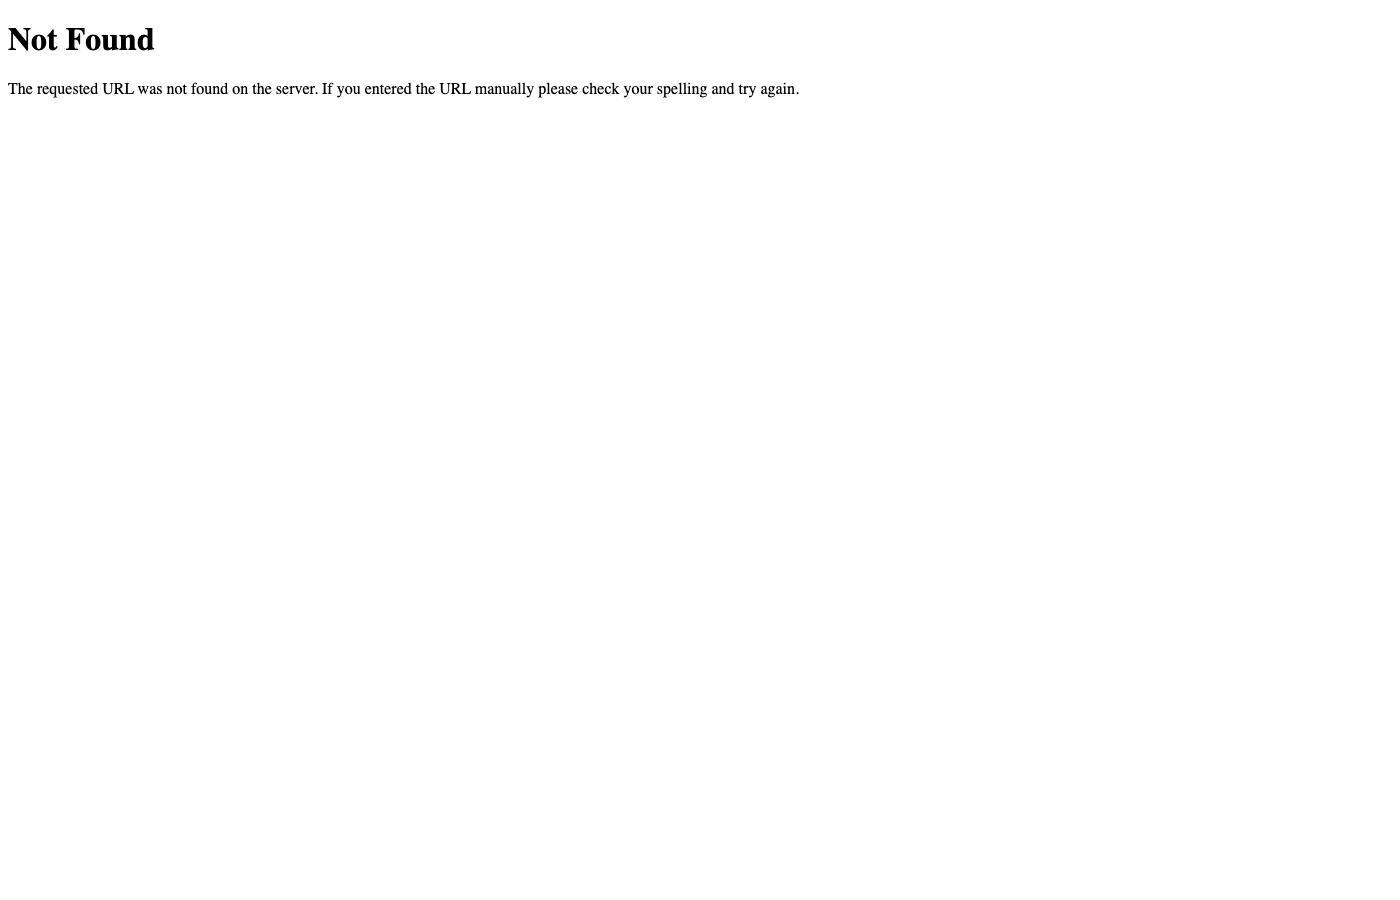
\includegraphics[width=\textwidth]{dashboard_main}
  \caption{Live dashboard (Prishtina): metric cards with trend indicators, AI Insights, Station Metadata, five live Chart.js plots, the Spark Aggregated Trends panel, and the recent alerts list.}
  \label{fig:dashboard}
\end{figure*}

\begin{itemize}
  \item \textbf{Time range selector}: 30\,min / 1\,h / 3\,h / 6\,h buttons control how much history is fetched. The API downsamples to 300 points for chart performance.
  \item \textbf{Station dropdown}: Shows city names (Prishtina, Peja, Prizren).
  \item \textbf{Live indicator}: Pulsing green dot confirms data is flowing.
  \item \textbf{Alert banner}: Shown when the most recent alert is less than 2~minutes old. Red for critical, amber for warning.
  \item \textbf{Metric cards}: Current value, weather icon, colour-coded top border, and trend arrow (↑/↓/→) comparing current to previous reading.
  \item \textbf{Charts}: Five live-updating line charts in a 3+2 grid: Temperature (°C), Humidity (\%), Pressure (hPa), Precipitation (mm/h), Wind Speed (m/s).
  \item \textbf{AI Insights panel}: Three live ML results (Section~\ref{sec:ai}).
  \item \textbf{Station Metadata panel}: City, GPS coordinates, altitude, sensors, installation date --- read from Cassandra.
  \item \textbf{Aggregated Trends panel}: A table of the most recent Spark 5-minute sliding windows (avg temperature/humidity/pressure, total precipitation, max wind, reading count), surfacing the output of Query~B directly in the UI.
  \item \textbf{Recent Alerts list}: Severity pills, timestamps, messages, and count badges.
\end{itemize}

Figure~\ref{fig:peja} shows the Peja station, where the AI has classified the
current condition as STORM and multiple threshold breaches are visible.

\begin{figure*}[t]
  \centering
  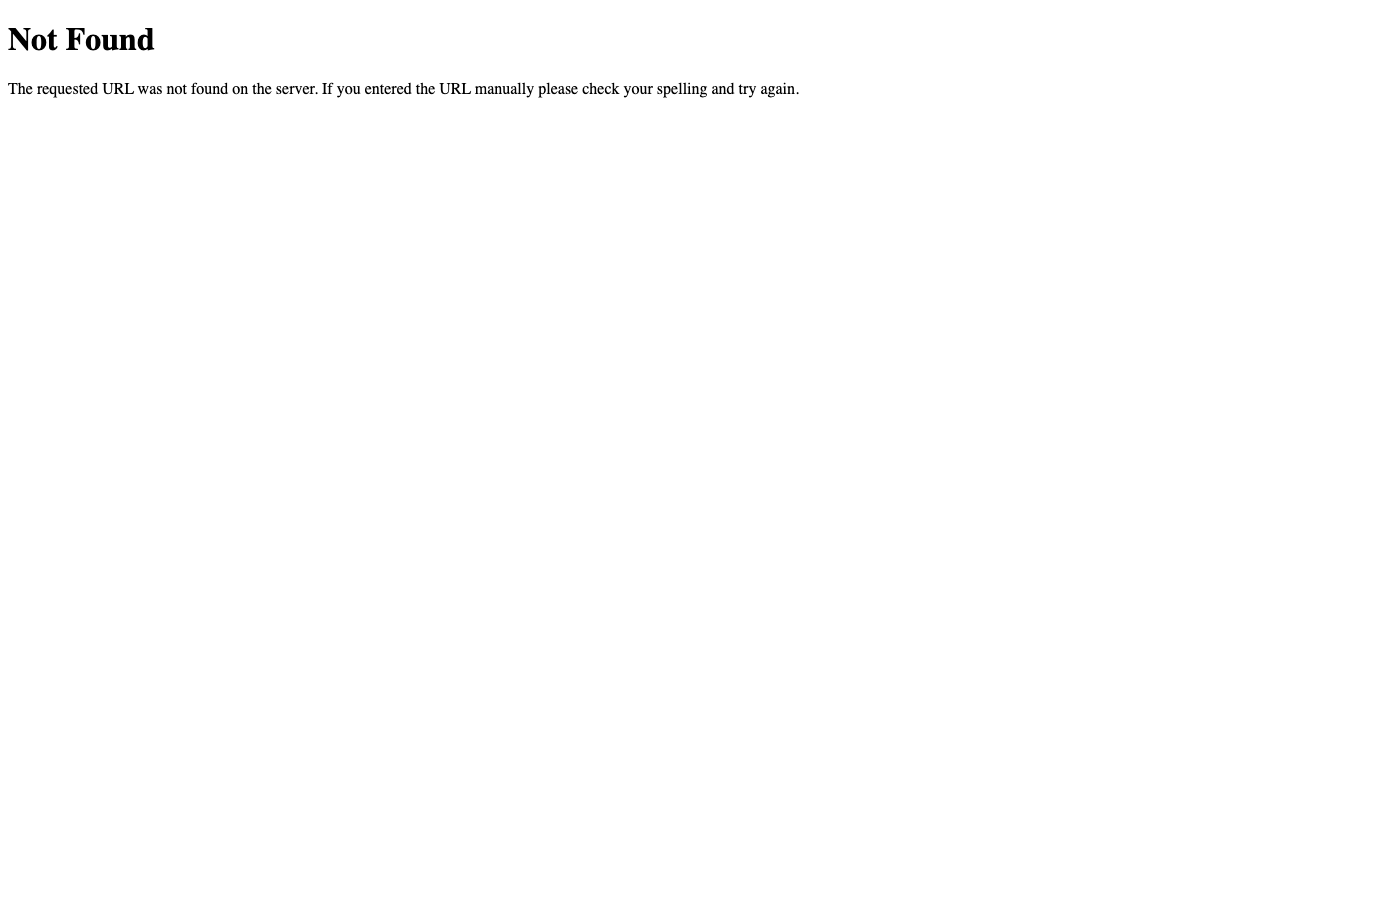
\includegraphics[width=\textwidth]{dashboard_anomaly}
  \caption{Peja station: the AI Insights panel reports a STORM condition; the alert count badges and recent-alerts list show real-time threshold breaches detected by Spark, alongside the live charts and aggregated-window trends.}
  \label{fig:peja}
\end{figure*}

\subsection{PDF Report Export}

The ``Export PDF'' button generates a downloadable A4 report without any external API:
station info, current conditions, statistics table (avg/min/max per parameter),
AI insights, alert summary table, and five embedded Matplotlib trend charts in a print-friendly light theme.

% ========================================================================
\section{Advanced Components}

\subsection{Artificial Intelligence Module}
\label{sec:ai}

Three fully local machine learning models are trained on 26\,280 rows of synthetic
history (one year at 10-minute intervals, generated by the same simulator). No
external API or internet connection is required.

\subsubsection{Model 1 --- Temperature Forecaster}
\textbf{Algorithm}: GradientBoostingRegressor (200 estimators, max depth 3).
\textbf{Features}: Lag values (temperature, humidity, pressure, wind speed) and
cyclical time encoding (hour-of-day and day-of-year as sine/cosine pairs).
\textbf{Result}: MAE of \textbf{0.37\,°C} on the held-out test set.

\subsubsection{Model 2 --- Anomaly Detector}
\textbf{Algorithm}: IsolationForest (150 estimators, contamination 2\,\%).
Enhanced with per-feature plausible range bounds (25\,\% margin beyond training extremes).
A reading is flagged if either the IsolationForest score or a per-feature range check fires,
with the specific out-of-range parameter reported.
This detects the 1\,\% injected sensor faults generated by the simulator.

\subsubsection{Model 3 --- Condition Classifier}
\textbf{Algorithm}: RandomForestClassifier (120 estimators).
\textbf{Labels}: \texttt{stable} / \texttt{storm} / \texttt{extreme},
derived from rule-based thresholds applied to the training data.
\textbf{Result}: 100\,\% accuracy on the test set.
The dashboard displays the class as a colour-coded badge (green / amber / red).

\subsection{Real-Time Alerting System}

Alerts are detected inside the Spark Streaming job --- not client-side. All thresholds
are defined in \texttt{config/project\_config.ini} under \texttt{[thresholds]}
and can be changed without touching code.

\begin{table}[H]
\centering
\caption{Alert thresholds by parameter}
\label{tab:thresholds}
\renewcommand{\arraystretch}{1.1}
\begin{tabular}{lcccc}
\toprule
\textbf{Parameter} & \textbf{W-Low} & \textbf{C-Low} & \textbf{W-High} & \textbf{C-High} \\
\midrule
Temperature (°C)    & $-5$  & $-12$ & 35   & 40   \\
Humidity (\%)       & ---   & ---   & 85   & 95   \\
Pressure (hPa)      & 995   & 980   & 1030 & 1040 \\
Precip.\ (mm/h)     & ---   & ---   & 15   & 30   \\
Wind (m/s)          & ---   & ---   & 14   & 20   \\
\bottomrule
\end{tabular}
\end{table}

Detected alerts are simultaneously written to the \texttt{weather\_alerts}
Cassandra table \emph{and} published to the \texttt{weather\_alerts} Kafka topic,
making them available to any downstream consumer (e.g.\ an SMS gateway).

\subsection{Performance Analysis and Optimization}

The benchmarking suite (\texttt{performance\_analysis/benchmark\_pipeline.py})
measures the actual live Docker stack --- not simulated data.

\subsubsection{Kafka Throughput}

\begin{figure}[H]
  \centering
  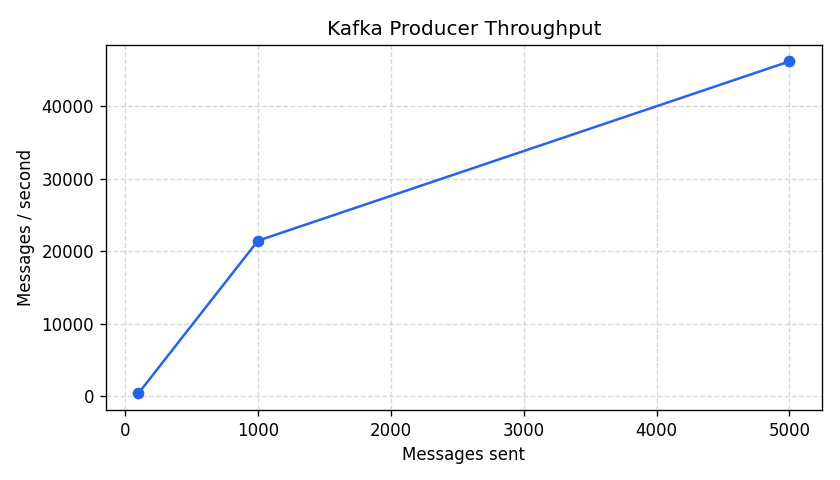
\includegraphics[width=\columnwidth]{kafka_throughput}
  \caption{Kafka producer throughput: approx.\ 46\,000 msg/s at 5\,000 messages}
  \label{fig:kafka}
\end{figure}

At 5\,000 messages, Kafka sustains approximately 46\,000~messages/second ---
far above the 90~readings/minute produced by the simulator,
demonstrating substantial headroom for scaling.

\subsubsection{Cassandra Write Optimization}

The key optimization is switching from sequential synchronous writes to concurrent
pipelined writes (\texttt{execute\_concurrent\_with\_args}, concurrency 64):

\begin{table}[H]
\centering
\caption{Cassandra write throughput}
\label{tab:cass}
\begin{tabular}{lrr}
\toprule
\textbf{Method} & \textbf{rows/s} & \textbf{gain} \\
\midrule
Sequential & 512 & --- \\
Concurrent & 14\,798 & \textbf{28.9×} \\
\bottomrule
\end{tabular}
\end{table}

\begin{figure}[H]
  \centering
  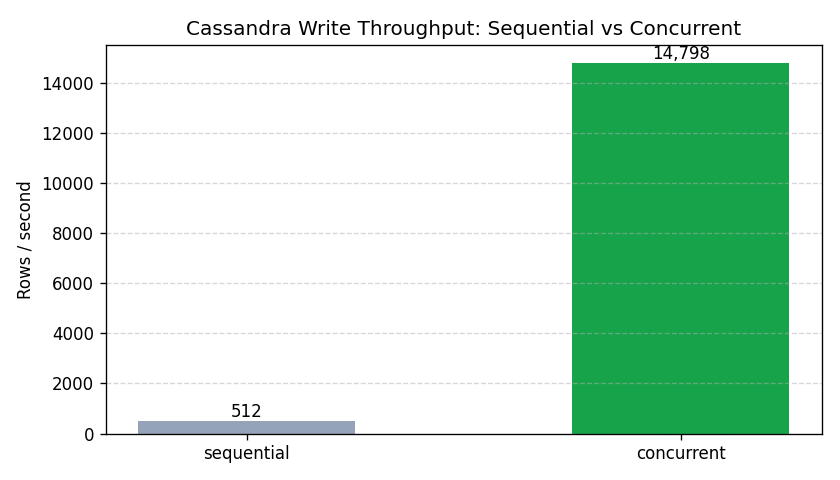
\includegraphics[width=\columnwidth]{cassandra_writes}
  \caption{Sequential (512 rows/s) vs.\ concurrent (14\,798 rows/s) writes}
  \label{fig:cassandra}
\end{figure}

Sequential writes pay one full network round-trip per insert.
Pipelining 64 in-flight writes saturates the connection and achieves a 28.9$\times$ improvement.

\subsubsection{End-to-End Latency}

The script measures produce-to-queryable latency through the full pipeline
(Kafka consumer + Spark micro-batch + Cassandra write). Typical observed latency
is 5--8~seconds, dominated by the 5-second Spark trigger interval.

% ========================================================================
\section{Results and Evaluation}

This section consolidates the measured evidence collected while the system ran
continuously, demonstrating that every stage of the pipeline functions
end-to-end under sustained load.

\subsection{Pipeline Throughput and Storage}

Table~\ref{tab:results} summarizes the data the live system accumulated across
the Cassandra tables during a representative multi-hour run, together with
the key performance figures.

\begin{table}[H]
\centering
\caption{Measured system results}
\label{tab:results}
\renewcommand{\arraystretch}{1.15}
\begin{tabular}{ll}
\toprule
\textbf{Metric} & \textbf{Measured value} \\
\midrule
Raw readings stored        & 4\,266 rows \\
Window aggregates stored   & 246 rows \\
Alerts detected \& stored  & 1\,032 rows \\
Stations seeded            & 3 \\
Producer emit rate         & 3 readings / 2\,s ($\approx$90/min) \\
Kafka throughput (peak)    & $\approx$46\,000 msg/s \\
Cassandra write gain       & 28.9$\times$ (512 $\rightarrow$ 14\,798 rows/s) \\
End-to-end latency         & 5--8\,s \\
Forecaster accuracy (MAE)  & 0.37\,°C \\
Classifier accuracy        & 100\,\% (test set) \\
\bottomrule
\end{tabular}
\end{table}

\subsection{Functional Verification}

Each pipeline stage was verified against live evidence rather than assumed:

\begin{itemize}
  \item \textbf{Ingestion}: producer logs confirm three keyed readings published
        to Kafka every 2~seconds.
  \item \textbf{Processing}: Spark batch logs report rows written and alerts
        raised per micro-batch (e.g.\ \emph{``Batch 1: wrote 9 reading(s),
        2 alert(s)''}), with a data-quality count when invalid readings are
        filtered.
  \item \textbf{Storage}: \texttt{cqlsh} queries confirm all five tables
        populate and that the latest-timestamp clustering returns the newest
        reading first.
  \item \textbf{Alerting}: the independent alerts consumer logs each breach it
        receives from the \texttt{weather\_alerts} topic, routes it by severity,
        and writes an audit record --- verified by matching row counts between
        \texttt{weather\_alerts} and \texttt{alert\_notifications}, confirming
        the pub/sub path end-to-end.
  \item \textbf{Visualization}: the dashboard renders all five charts, the
        aggregated-window panel, AI insights, and the live alert banner.
\end{itemize}

\subsection{Automated Testing}

A \texttt{pytest} suite (15 tests, all passing) validates the components that are
pure logic and therefore unit-testable without the running cluster:

\begin{itemize}
  \item \textbf{Simulator (8 tests)}: one reading per station, all fields
        present, humidity clamping for normal readings, physical plausibility of
        non-anomalous readings, non-negative precipitation, deterministic output
        for a fixed seed, divergence across seeds, and a warmer-summer-than-winter
        seasonal baseline.
  \item \textbf{Thresholds and validation (7 tests)}: every parameter has a
        threshold, threshold bands are monotonic (\texttt{crit\_low} $\le$
        \texttt{warn\_low}, \texttt{warn\_high} $\le$ \texttt{crit\_high}),
        validation bounds satisfy \texttt{min} $<$ \texttt{max}, and the
        severity-decision rule returns the correct level (including
        critical-over-warning priority and one-sided thresholds).
\end{itemize}

The tests encode the contracts the rest of the pipeline depends on, so a
regression in the simulator physics or the alert rule is caught immediately.

% ========================================================================
\section{Conclusions and Recommendations}

\subsection{Achievements}

The project delivered a fully functional, containerized, real-time IoT weather monitoring system. Key results:

\begin{itemize}
  \item Complete end-to-end pipeline starting with one command.
  \item Physics-based simulator producing temporally correlated, meaningful training data for AI.
  \item A Spark data-validation stage implementing a medallion (bronze/silver) pattern so faulted readings never skew the aggregates.
  \item Real-time alerting inside Spark with dual output to Cassandra and Kafka, plus a second independent consumer that routes alerts by severity.
  \item Three fully local AI models with no external API dependency.
  \item Genuine pipeline benchmarks: 28.9$\times$ Cassandra write optimization, 46\,000~msg/s Kafka throughput.
  \item A resilient, self-healing Kafka consumer (generous timeouts + clean-restart recovery), a 15-test automated suite, and PDF report export directly from the dashboard.
\end{itemize}

\subsection{Challenges Encountered}

\begin{itemize}
  \item \textbf{Spark query contention}: Two concurrent streaming queries with default settings caused stalls. Resolved with FAIR scheduler, \texttt{local[6]}, reduced shuffle partitions, and combining raw + alerting into one \texttt{foreachBatch}.
  \item \textbf{Library version conflict}: WeasyPrint 59.0 was incompatible with pydyf 0.11.0. Pinning WeasyPrint to 62.3 resolved the \texttt{TypeError}. Highlighted the importance of fully pinning all dependency versions.
  \item \textbf{Schema consistency}: Any mismatch between the JSON schema, the Spark \texttt{StructType}, and the Cassandra table definition silently drops data. A single shared configuration file reduced this risk.
  \item \textbf{Cassandra key design}: The \texttt{CLUSTERING ORDER BY (ts DESC)} clause physically stores rows in descending time order, making the dashboard's \texttt{LIMIT~1} query a single I/O operation regardless of partition size.
  \item \textbf{Streaming reliability}: The processor would intermittently go silent. Logs traced it to a transient Kafka offset-fetch timeout (\texttt{TimeoutException ... before the position for partition ... could be determined}) that hard-killed the query --- not memory pressure. The fix was twofold: generous Kafka consumer timeouts plus \texttt{failOnDataLoss=false} to prevent the crash, and clearing the checkpoint on every start so the \texttt{restart: unless-stopped} policy always recovers cleanly from the live tail (an attempt to persist checkpoints instead left the stream wedged on poisoned state after a crash).
\end{itemize}

\subsection{Recommendations}

\begin{itemize}
  \item Replace 4-second HTTP polling with WebSocket push for lower-latency updates.
  \item Deploy Kafka and Cassandra as multi-node clusters for true fault tolerance.
  \item Use a proper cluster manager (Kubernetes, YARN) instead of \texttt{local[6]}.
  \item Integrate the \texttt{weather\_alerts} Kafka topic with an SMS or email gateway for active operator notifications.
  \item Train AI models on real Kosovo historical weather data for improved forecast accuracy.
\end{itemize}

\end{document}
